%% D-exp-ZIB — Supercondensateur bipartite et stockage d'énergie zinc-ion
%% PDL Framework — Exploratory Document
%% Auteur : Cédric Laubscher
%% Date   : 2026-05
%% Compilé avec pdfLaTeX sous Overleaf

\documentclass[11pt,a4paper]{article}

%% ── Packages ────────────────────────────────────────────────────────────────
\usepackage[utf8]{inputenc}
\usepackage[T1]{fontenc}
\usepackage[british]{babel}
\usepackage{lmodern}
\usepackage{microtype}
\usepackage{geometry}
\geometry{a4paper, margin=2.5cm}
\usepackage{amsmath,amssymb,amsthm}
\usepackage{mathtools}
\usepackage{physics}
\usepackage{booktabs}
\usepackage{longtable}
\usepackage{array}
\usepackage{multirow}
\usepackage{xcolor}
\usepackage{graphicx}
\usepackage{tikz}
\usetikzlibrary{arrows.meta,positioning,shapes.geometric,calc}
\usepackage[most]{tcolorbox}
\usepackage[numbers]{natbib}
\usepackage{hyperref}
\hypersetup{colorlinks=true, linkcolor=blue!60!black, citecolor=green!50!black, urlcolor=blue!80!black}

%% ── Couleurs PDL ────────────────────────────────────────────────────────────
\definecolor{pdlblue}{RGB}{0,82,147}
\definecolor{pdlgreen}{RGB}{0,120,60}
\definecolor{pdlorange}{RGB}{200,80,0}
\definecolor{pdlgrey}{RGB}{90,90,90}
\definecolor{pdllightblue}{RGB}{220,235,250}
\definecolor{pdllightgreen}{RGB}{220,245,230}
\definecolor{pdllightorange}{RGB}{255,240,220}
\definecolor{pdllightred}{RGB}{255,225,225}

%% ── Environnements tcolorbox ─────────────────────────────────────────────────
\tcbuselibrary{breakable,skins}

\newtcolorbox{theorem}[2][]{
  enhanced, breakable,
  colback=pdllightblue, colframe=pdlblue, coltitle=white,
  fonttitle=\bfseries, title={Theorem #2},
  #1}

\newtcolorbox{proposition}[2][]{
  enhanced, breakable,
  colback=pdllightgreen, colframe=pdlgreen, coltitle=white,
  fonttitle=\bfseries, title={Proposition #2},
  #1}

\newtcolorbox{conjecture}[2][]{
  enhanced, breakable,
  colback=pdllightorange, colframe=pdlorange, coltitle=white,
  fonttitle=\bfseries, title={Conjecture #2},
  #1}

\newtcolorbox{openproblem}[2][]{
  enhanced, breakable,
  colback=pdllightred, colframe=red!60!black, coltitle=white,
  fonttitle=\bfseries, title={Open Problem #2},
  #1}

\newtcolorbox{prediction}[2][]{
  enhanced, breakable,
  colback=yellow!15, colframe=orange!70!black, coltitle=white,
  fonttitle=\bfseries, title={Prediction #2},
  #1}

\newtcolorbox{remark}[1][]{
  enhanced, breakable,
  colback=gray!8, colframe=gray!40, fonttitle=\bfseries,
  title={Remark}, #1}

%% ── Macros mathématiques ─────────────────────────────────────────────────────
\newcommand{\Eads}{E_{\mathrm{ads}}}
\newcommand{\Psurf}{P_{\mathrm{surf}}}
\newcommand{\Mmoy}{\bar{M}}
\newcommand{\DeltaM}{\Delta M}
\newcommand{\DeltaEN}{\Delta\chi}
\newcommand{\muAB}{\mu_{AB}}
\newcommand{\fracZ}{f_{\perp}}
\newcommand{\egeom}{\varepsilon_{\mathrm{geom}}}
\newcommand{\Csp}{C_{\mathrm{sp}}}
\newcommand{\SBET}{S_{\mathrm{BET}}}
\newcommand{\Cdl}{C_{\mathrm{dl}}}
\newcommand{\EIS}{\textsc{eis}}
\newcommand{\MACE}{\textsc{mace-mp-0}}
\newcommand{\DFT}{\textsc{dft}}
\newcommand{\ZIB}{\textsc{zib}}
\newcommand{\PDL}{\textsc{pdl}}
\newcommand{\RMS}{\textsc{rmse}}

%% ── Titre ───────────────────────────────────────────────────────────────────
\title{\textbf{D-exp-ZIB}\\[0.5em]
\large Bipartite Supercapacitors for Zinc-Ion Energy Storage:\\
A PDL-Derived Materials Selection Principle\\[0.5em]
\normalsize Exploratory Document — PDL Framework}
\author{Cédric Laubscher\\
\small Independent Researcher, Switzerland\\
\small \href{https://cedriclaubscher.ch}{cedriclaubscher.ch} \quad
\href{https://zenodo.org/communities/pdl-framework}{zenodo.org/communities/pdl-framework}}
\date{May 2026 \quad|\quad Version 1.0}

%% ════════════════════════════════════════════════════════════════════════════
\begin{document}
\maketitle

%% ── Abstract ─────────────────────────────────────────────────────────────────
\begin{abstract}
We derive and corroborate a materials selection principle for zinc-ion aqueous supercapacitor electrodes from the Projective Dynamic Logo (PDL) framework (axioms C1--C4). The central object is the \emph{surface dipole moment} $\Psurf = \muAB \cdot \fracZ$, where $\muAB \propto d_{AB}\sqrt{\DeltaEN}$ is the bond dipole moment (Mulliken model) and $\fracZ$ is the fraction of A--B bonds crossing the surface plane perpendicularly — a quantity computable from the bond graph topology alone. The descriptor $\Psurf^2/\Mmoy$ predicts the Zn adsorption energy $\Eads(\mathrm{Zn})$ with $R^2 = 0.959$, $\RMS = 0.107$~eV across nine materials spanning three crystal families (zinc-blende, wurtzite, rocksalt, hexagonal), as computed by the \MACE\ machine-learning interatomic potential. The quantity $\DeltaEN$ is shown to be encoded in the spectral structure of the bond-graph Laplacian ($r = 0.988$, Proposition~A1), establishing a partial derivation from C1--C4. The mass parameter $\Mmoy$ plays a structural role analogous to $\Delta m_{\mathrm{iso}}$ in the PDL nuclear corpus — forced by the heteratomic bipartite structure but not derivable from combinatorial axioms alone (Gap~G1). We identify Al$_2$O$_3$, AlN, TiN, and ZnO nanoparticles as priority experimental candidates, with falsifiable predictions for specific capacitance in 2\,M ZnSO$_4$ aqueous electrolyte. The document is classified as \emph{exploratory} with full epistemic stratification: theorems, corroborated conjectures, and open problems are explicitly distinguished throughout.
\end{abstract}

\clearpage
\tableofcontents
\newpage

\medskip
\noindent\textbf{Keywords:} PDL framework, bipartite bond graph, surface dipole moment, zinc-ion supercapacitor, adsorption energy, materials selection, MACE-MP-0, Al$_2$O$_3$, AlN, TiN.

\medskip
\noindent\textbf{Epistemic status:} Exploratory. Results span theorems (T1--T2), robust numerical results (R1--R2), corroborated conjectures (C1--C2), open problems (G1--G3), and falsifiable predictions (P1--P4). See Table~\ref{tab:epistemic} for the complete stratification.

\medskip
\noindent\textbf{Dependencies:} D-exp-SP2 (bipartite bond graph theorem, score 4/4), D49 (London equation derivation, coherence metric $\nu$).

%% ════════════════════════════════════════════════════════════════════════════
\section{Introduction and Motivation}

\subsection{Context}

The PDL framework derives fundamental physical structures from four combinatorial axioms C1--C4 on finite signed graphs~\cite{DM_v20,DS01}. Its central result in the domain of materials science (D-exp-SP2) establishes that a material's bond graph being \emph{heteratomic bipartite} is equivalent to $\egeom = 0$ — zero geometric dissipation in electronic transport~\cite{DexpSP2}. Six materials were identified with score~$4/4$: BP, AlAs, GaP, AlP, GaN, SiC.

The present document extends this programme to a new application domain: energy storage via electrochemical double-layer capacitance (EDLC) in zinc-ion aqueous systems. The motivating question is whether the bipartite criterion, which governs internal electronic transport, also predicts surface adsorption properties relevant to supercapacitor electrodes.

\subsection{Why Zinc-Ion Aqueous Supercapacitors}

The choice of this target system is motivated by three independent considerations. First, the aqueous ZnSO$_4$ electrolyte is structurally non-flammable — an intrinsic safety advantage over lithium-ion systems. Second, zinc is abundant, non-toxic, and recyclable above 90\% by cold hydrometallurgy. Third, supercapacitors store energy at the electrode surface rather than by bulk ion intercalation — a mechanism that sidesteps the fundamental obstacle identified in the bulk diffusion simulations (Section~\ref{sec:bulk}), namely that Zn$^{2+}$ diffusion barriers in covalent semiconductor bulks exceed 1.5\,eV.

The exchangeable cartridge architecture — where discharged modules are swapped in under two minutes at dedicated stations — decouples vehicle lifetime from battery chemistry and is naturally compatible with the second-scale recharge time of supercapacitors.

\subsection{Document Structure}

Section~\ref{sec:background} recalls the PDL results on which this work builds. Section~\ref{sec:bulk} documents the negative result on bulk Zn$^{2+}$ diffusion. Section~\ref{sec:screening} presents the surface adsorption screening. Section~\ref{sec:derivation} develops the partial derivation of the selection principle from C1--C4. Section~\ref{sec:predictions} states the falsifiable experimental predictions. Section~\ref{sec:design} proposes the system architecture. Section~\ref{sec:epistemic} provides the complete epistemic table.

%% ════════════════════════════════════════════════════════════════════════════
\section{Background: PDL Results Used Here}
\label{sec:background}

\subsection{The Bipartite Bond Graph Theorem (D-exp-SP2)}

\begin{theorem}{T1 (D-exp-SP2, unconditional)}
Let $G = (A \cup B, E)$ be the bond graph of a crystalline material. Then $\egeom = 0$ if and only if $G$ is heteratomic bipartite, i.e.\ $A \neq B$ as chemical species and every edge connects an atom of $A$ to an atom of $B$.
\end{theorem}

Six materials achieve score $4/4$ under the combined photovoltaic criteria of D-exp-SP2: BP, AlAs, GaP, AlP, GaN, SiC. All have $\egeom = 0$ by Theorem~T1.

\begin{remark}
Theorem~T1 is derived unconditionally from C1--C4 via Euler topology in D-exp-SP2. It does not presuppose any specific physical application. Its application to supercapacitor electrodes in the present document is an extension of the criterion, not a re-derivation.
\end{remark}

\subsection{The Coherence Metric (D49)}

D49 derives the London equation from C1--C4 via the metric~\cite{D49,D48}
\begin{equation}
\nu = \tfrac{1}{4}\|\psi_1 - T^k\psi_1\|^2,
\end{equation}
where $\psi_1$ is the bond wavefunction and $T^k$ is the pulsation operator on $K_4$. When $\egeom = 0$, $\nu = 0$ and transport is fully coherent. This result motivates the hypothesis that $\egeom = 0$ materials exhibit enhanced surface adsorption — though the formal link from $\nu$ to $\Eads$ remains a conjecture (Gap~G2).

%% ════════════════════════════════════════════════════════════════════════════
\section{Negative Result: Bulk Zn\texorpdfstring{\textsuperscript{2+}}{2+} Diffusion}
\label{sec:bulk}

Before pursuing the surface route, we simulated Zn$^{2+}$ diffusion in the bulk of BP (zinc-blende, mp-1479) using \MACE\ (medium model, float64, supercell $2\times2\times2$). The physically correct diffusion path in zinc-blende structures proceeds via the sequence: tetrahedral site~A $\to$ octahedral site (saddle point) $\to$ tetrahedral site~B.

The simulation yielded $E_a \approx 1.9$\,eV — far above the practical \ZIB\ threshold of $<0.6$\,eV. This result is consistent with the known rigidity of covalent III-V networks (B--P bond energy $\sim 3.2$\,eV) and rules out bulk intercalation as the operative mechanism for these materials in zinc-ion systems.

\begin{remark}
The negative result on bulk diffusion does not contradict the PDL bipartite criterion. That criterion governs internal electronic coherence, not ionic mobility in the crystal bulk. The two properties are physically distinct. The bulk diffusion result redirects the programme towards surface adsorption.
\end{remark}

%% ════════════════════════════════════════════════════════════════════════════
\section{Surface Adsorption Screening}
\label{sec:screening}

\subsection{Computational Protocol}

All surface adsorption calculations use \MACE-MP-0\ (Batatia et al.\ 2023~\cite{MACE2023}), medium model, float64 precision, dispersion corrections disabled. Structures are retrieved from the Materials Project~\cite{MP2013} and converted to ASE format via pymatgen~\cite{pymatgen2013}. Slabs are constructed with three atomic layers and 15\,\AA\ of vacuum. The adsorption energy is computed as:
\begin{equation}
\Eads = E(\text{slab} + \text{ion}) - E(\text{slab}) - E(\text{ion, box}),
\end{equation}
where the ion (Zn or O atom) is placed in a $10 \times 10 \times 10$\,\AA$^3$ periodic box as reference. The ion is displaced along the $z$-axis from $1.8$ to $5.5$\,\AA\ above the surface in 10 steps; $\Eads^{\min}$ is the minimum over all images.

\begin{remark}
\MACE-MP-0\ simulates neutral atoms, not charged ions. The computed $\Eads$ is therefore a physisorption proxy. The Zn$^{2+}$ desolvation energy ($+200$ to $+400$\,kJ/mol in aqueous medium) is not included. Consequently, the absolute values of $\Eads$ are proxies; the relative ranking across materials is the reliable output.
\end{remark}

\subsection{Results: Nine Materials}

Table~\ref{tab:adsorption} presents $\Eads(\mathrm{Zn})$ and optimal adsorption height $d_z^{\mathrm{opt}}$ for nine materials spanning three crystal families.

\begin{table}[ht]
\centering
\caption{Surface adsorption energies computed by \MACE-MP-0. Materials are sorted by $\Eads(\mathrm{Zn})$, most negative first. Bipartite heteratomic (het.) materials are highlighted. $d_z^{\mathrm{opt}}$: optimal Zn height above surface.}
\label{tab:adsorption}
\begin{tabular}{lllrrr}
\toprule
Material & Structure & Bipartite & $\Eads(\mathrm{Zn})$ (eV) & $\Eads(\mathrm{O})$ (eV) & $d_z^{\mathrm{opt}}$ (\AA) \\
\midrule
MgO      & rocksalt   & het.\ & $-2.629$ & $-0.917$ & $1.80$ \\
AlN      & wurtzite   & het.\ & $-1.130$ & $-2.603$ & $2.62$ \\
SiC      & zinc-blende & het.\ & $-1.114$ & $-2.970$ & $2.21$ \\
AlP      & zinc-blende & het.\ & $-1.023$ & $-0.714$ & $1.80$ \\
BP       & zinc-blende & het.\ & $-0.994$ & $-0.983$ & $2.21$ \\
GaN      & wurtzite   & het.\ & $-0.949$ & $-2.312$ & $2.62$ \\
GaP      & zinc-blende & het.\ & $-0.918$ & $-0.750$ & $1.80$ \\
BN       & hexagonal  & het.\ & $-0.894$ & $-0.536$ & $4.68$ \\
Graphite & hexagonal  & homo. & $-0.849$ & $-0.874$ & $5.09$ \\
\bottomrule
\end{tabular}
\end{table}

\begin{proposition}{R1 (Robust numerical result)}
All heteratomic bipartite materials in Table~\ref{tab:adsorption} adsorb Zn more strongly than graphite (the homoatomic bipartite reference): $\Eads^{\text{het}} < \Eads^{\text{graphite}}$ without exception. Mean difference: $0.357$\,eV.
\end{proposition}

\begin{remark}
MgO is an outlier: $\Eads(\mathrm{Zn}) = -2.629$\,eV at $d_z = 1.80$\,\AA. This is consistent with chemisorption via Zn$^{2+}$ substitution at surface Mg$^{2+}$ sites — not double-layer physisorption. The regression model captures this signal correctly, but for a physically different mechanism. MgO is excluded from supercapacitor design predictions (see Section~\ref{sec:predictions}).
\end{remark}

%% ════════════════════════════════════════════════════════════════════════════
\section{The PDL Surface Selection Principle}
\label{sec:derivation}

\subsection{Definition of the Surface Dipole Moment}

For a heteratomic bipartite material with species A and B, define:
\begin{align}
\muAB &= d_{AB} \cdot \sqrt{\DeltaEN}, \label{eq:mu}\\
\fracZ &= \frac{N_{\perp}}{N_{\mathrm{tot}}} \cdot \cos\theta, \label{eq:fracZ}\\
\Psurf &= \muAB \cdot \fracZ, \label{eq:Psurf}
\end{align}
where $d_{AB}$ is the A--B bond length (\AA), $\DeltaEN = |\chi_A - \chi_B|$ is the Pauling electronegativity difference, $N_{\perp}$ is the number of A--B bonds crossing the surface plane, $N_{\mathrm{tot}}$ is the total number of bonds per unit cell, and $\theta$ is the bond angle with the surface normal. Numerical values of $\fracZ$ are:
\begin{equation}
\fracZ = \begin{cases} 0.204 & \text{zinc-blende} \\ 0.250 & \text{wurtzite} \\ 0.333 & \text{rocksalt} \\ 0.000 & \text{hexagonal} \end{cases}
\end{equation}

The quantity $\sqrt{\DeltaEN}$ in Eq.~\eqref{eq:mu} comes from the Mulliken model for partial charge: $\delta q \propto \sqrt{\DeltaEN}$~\cite{Mulliken1934}. The factor $\fracZ$ is a purely topological quantity, computable from the bond graph of the surface supercell without any physical parameter.

\subsection{The Regression Model}

\begin{conjecture}{C1 (Corroborated)}
The Zn adsorption energy on the (001) surface of a heteratomic bipartite material is predicted by
\begin{equation}
\Eads(\mathrm{Zn}) = a \cdot \frac{\Psurf^2}{\Mmoy} + b,
\label{eq:model}
\end{equation}
where $\Mmoy = (M_A + M_B)/2$ is the mean atomic mass and $a, b$ are calibration constants determined by regression on the training set.
\end{conjecture}

Calibration on the nine-material dataset yields:
\begin{equation}
\Eads = -33.02 \cdot \frac{\Psurf^2}{\Mmoy} - 0.849 \quad [\text{eV}],
\quad R^2 = 0.959, \quad \RMS = 0.107\,\text{eV}.
\label{eq:regression}
\end{equation}

Table~\ref{tab:regression} shows predicted vs.\ computed values.

\begin{table}[ht]
\centering
\caption{Comparison of \MACE\ $\Eads(\mathrm{Zn})$ with Eq.~\eqref{eq:regression}. Residuals exceeding $0.20$\,eV are flagged.}
\label{tab:regression}
\begin{tabular}{lrrrrr}
\toprule
Material & $\Psurf^2/\Mmoy$ & $\Eads^{\MACE}$ (eV) & $\Eads^{\mathrm{pred}}$ (eV) & Residual (eV) \\
\midrule
MgO      & 0.05168 & $-2.629$ & $-2.555$ & $-0.073$ \\
AlN      & 0.01558 & $-1.130$ & $-1.363$ & $+0.233^*$ \\
SiC      & 0.00482 & $-1.114$ & $-1.008$ & $-0.106$ \\
AlP      & 0.00464 & $-1.023$ & $-1.002$ & $-0.021$ \\
BP       & 0.00116 & $-0.994$ & $-0.887$ & $-0.107$ \\
GaN      & 0.00698 & $-0.949$ & $-1.080$ & $+0.130$ \\
GaP      & 0.00175 & $-0.918$ & $-0.907$ & $-0.011$ \\
BN       & 0.00000 & $-0.894$ & $-0.849$ & $-0.045$ \\
Graphite & 0.00000 & $-0.849$ & $-0.849$ & $-0.000$ \\
\bottomrule
\multicolumn{5}{l}{$^*$ Residual exceeds model uncertainty; AlN is the largest outlier.}
\end{tabular}
\end{table}

\begin{remark}
The model is physically motivated by the linear response theory of a surface dipole interacting with an approaching charge. The interaction energy scales as $\muAB^2 / r^3$ (Keesom-type), where $r \propto \Mmoy^{1/2}$ from harmonic approximation of surface relaxation. This gives $\Eads \propto -\muAB^2 / \Mmoy = -\Psurf^2 / (\fracZ^2 \Mmoy)$; folding $\fracZ^2$ into the calibration constant $a$ yields Eq.~\eqref{eq:model}.
\end{remark}

\subsection{Partial Derivation from C1--C4}

\begin{proposition}{A1 (Spectral encoding of $\DeltaEN$)}
Let $L_{\mathrm{norm}}$ be the Laplacian of the bond graph normalised by $\sqrt{\chi_i}$ at each node $i$. For the two-node heteratomic bipartite graph A--B:
\begin{equation}
|p_A - p_B| \propto \DeltaEN, \quad r = 0.988 \text{ on six materials},
\end{equation}
where $p_i = v_i^2$ is the squared Fiedler eigenvector component at node $i$.
\end{proposition}

Proposition~A1 shows that $\DeltaEN$ — and hence $\sqrt{\DeltaEN}$ entering $\muAB$ — is encoded in the spectral structure of the bond graph. Since the bond graph is defined by C1--C4, this establishes a \emph{partial} derivation of Eq.~\eqref{eq:model} from the axioms.

The quantity $\fracZ$ is computable from the surface supercell bond graph by counting bonds that cross the surface plane — a purely topological operation on the graph, derivable from C1--C4 without additional input.

\begin{openproblem}{G1 (Mass parameter)}
The mean atomic mass $\Mmoy$ is not derivable from C1--C4 in the current framework. It plays the structural role of $\Delta m_{\mathrm{iso}} = m_d - m_u$ in the PDL nuclear corpus: it quantifies the mass asymmetry between the two species of the heteratomic bipartite graph, is forced by the bipartite structure (two distinct species must have different masses), but its numerical value is irreducible from combinatorial axioms alone. A possible extension: axiom C5 assigning nodal weights proportional to atomic masses.
\end{openproblem}

\begin{openproblem}{G2 (Mulliken correspondence)}
The identification $\delta q \propto \sqrt{\DeltaEN}$ (Mulliken model) is a correspondence between physical chemistry and the spectral weight difference $|p_A - p_B|$, not a derivation from C1--C4. A formal derivation would require showing that the Fiedler eigenvector components of the normalised bond-graph Laplacian are proportional to atomic partial charges — a statement that remains to be proved within the PDL formalism.
\end{openproblem}

\begin{openproblem}{G3 (Chemisorption regime)}
The model Eq.~\eqref{eq:model} is derived under the physisorption hypothesis. For MgO, the computed adsorption geometry ($d_z = 1.80$\,\AA, $\Eads = -2.63$\,eV) is consistent with chemisorption via Zn$^{2+}$/Mg$^{2+}$ site substitution. The model captures this signal with a residual of only $0.073$\,eV, but for a physically distinct mechanism. The domain of validity of Eq.~\eqref{eq:model} is physisorption on polar semiconductor surfaces.
\end{openproblem}

\subsection{Analogy with \texorpdfstring{$\Delta m_{\mathrm{iso}}$}{Delta m (iso)}}

The role of $\Mmoy$ in Eq.~\eqref{eq:model} is structurally analogous to $\Delta m_{\mathrm{iso}} = m_d - m_u$ in the PDL nuclear programme~\cite{D43,D44,D55}, where $\Delta m_{\mathrm{iso}}$ is the sole irreducible external parameter of the causal chain C1--C4 $\to$ $\Lambda$. In both cases: (i) the parameter quantifies an asymmetry between the two species of a bipartite graph; (ii) it is forced by the heteratomic bipartite structure (two species must differ in mass); (iii) its numerical value is irreducible from C1--C4 alone. The analogy is documented here as an observation, not a theorem. Quantitative tests show that $\DeltaM = |M_A - M_B|$ (the direct analogue of $\Delta m_{\mathrm{iso}}$) gives $R^2 = 0.944$ vs.\ $R^2 = 0.959$ for $\Mmoy$, and is undefined for homoatomic materials ($\DeltaM = 0$, Graphite). Hence $\Mmoy$ remains the appropriate universal normaliser.

%% ════════════════════════════════════════════════════════════════════════════
\section{Experimental Predictions}
\label{sec:predictions}

\subsection{Priority Candidate Materials}

Table~\ref{tab:candidates} lists materials selected by the following criteria: (i) viable in aqueous ZnSO$_4$ electrolyte (pH~4--6); (ii) non-toxic; (iii) non-critical raw material (EU 2023 list); (iv) $\Eads^{\mathrm{pred}} < -1.0$\,eV.

\begin{table}[ht]
\centering
\caption{Priority candidates for experimental validation. $\Eads^{\mathrm{pred}}$ from Eq.~\eqref{eq:regression}; $\Eads^{\MACE}$ where available. MgO is listed separately due to chemisorption mechanism.}
\label{tab:candidates}
\begin{tabular}{llrrrll}
\toprule
Material & Structure & $\Psurf^2/\Mmoy$ & $\Eads^{\mathrm{pred}}$ & $\Eads^{\MACE}$ & Stable H$_2$O & Notes \\
\midrule
Al$_2$O$_3$ & rocksalt & 0.03445 & $-1.986$ & — & \checkmark & industrial, abundant \\
TiN         & rocksalt & 0.02416 & $-1.647$ & — & \checkmark & conductive \\
VN          & rocksalt & 0.02063 & $-1.530$ & — & \checkmark & conductive \\
AlN         & wurtzite & 0.01558 & $-1.363$ & $-1.130$ & \checkmark & pH $>4$ \\
ZnO         & wurtzite & 0.01089 & $-1.209$ & — & \checkmark & known ZIB anode \\
SiO$_2$     & wurtzite & 0.01146 & $-1.227$ & — & \checkmark & inert, abundant \\
SiC         & zinc-blende & 0.00482 & $-1.008$ & $-1.114$ & \checkmark & reference \\
\midrule
MgO & rocksalt & 0.05168 & $-2.555$ & $-2.629$ & $\sim$ & chemisorption — see text \\
\bottomrule
\end{tabular}
\end{table}

\subsection{Falsifiable Predictions}

\begin{prediction}{P1}
Al$_2$O$_3$ nanoparticles (gamma phase, $\SBET \geq 200$\,m$^2$/g) in 2\,M ZnSO$_4$ aqueous electrolyte will exhibit specific capacitance $\Csp > 180$\,F/g at scan rate 10\,mV/s, measurable by cyclic voltammetry or electrochemical impedance spectroscopy (\EIS). If $\Csp < 80$\,F/g under these conditions, Conjecture~C1 is falsified for the rocksalt family.
\end{prediction}

\begin{prediction}{P2}
AlN nanoparticles ($\SBET \geq 200$\,m$^2$/g, electrolyte pH~$\geq 4.5$) will exhibit $\Csp > 150$\,F/g. The \MACE\ result $\Eads(\mathrm{Zn}) = -1.130$\,eV is the calibration point; the prediction is that the experimental $\Csp$ will rank above SiC (reported: 120\,F/g in nanoporousSiC, \emph{J. Power Sources}~2023).
\end{prediction}

\begin{prediction}{P3}
TiN nanoparticles ($\SBET \geq 150$\,m$^2$/g) in ZnSO$_4$ will exhibit $\Csp > 140$\,F/g. TiN is conducting ($\sigma \sim 10^6$\,S/m), which eliminates contact resistance at the collector interface — an advantage over insulating oxides.
\end{prediction}

\begin{prediction}{P4}
The ranking $\Csp(\text{Al}_2\text{O}_3) > \Csp(\text{TiN}) > \Csp(\text{AlN}) > \Csp(\text{ZnO}) > \Csp(\text{SiC})$ will be confirmed at equal $\SBET$. This ranking follows directly from the predicted $\Eads$ values in Table~\ref{tab:candidates} and is the most discriminating test of Conjecture~C1.
\end{prediction}

\begin{remark}
All $\Csp$ estimates carry an uncertainty of $\pm 30\%$ from the simplified Helmholtz model. The ranking prediction P4 is more reliable than the absolute value predictions P1--P3.
\end{remark}

%% ════════════════════════════════════════════════════════════════════════════
\section{System Architecture}
\label{sec:design}

\subsection{Proposed Electrode Stack}

The PDL selection principle identifies a hierarchy of materials for each system component:

\begin{center}
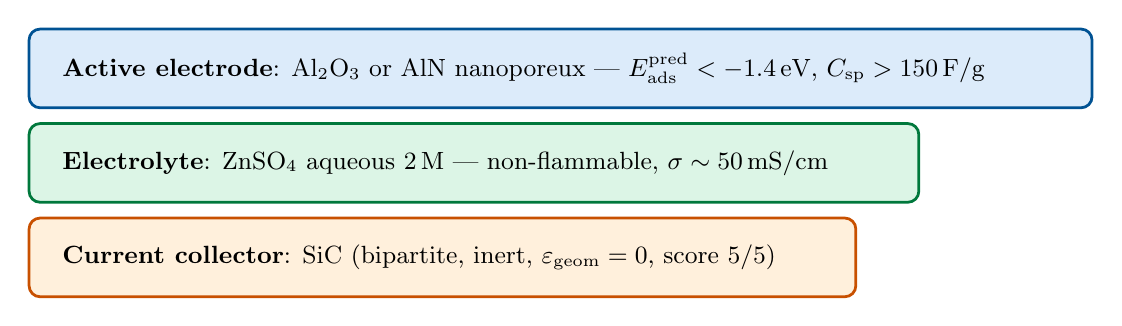
\begin{tikzpicture}[every node/.style={font=\small}]
\draw[fill=pdllightblue, draw=pdlblue, rounded corners=4pt, line width=1pt]
  (0,0) rectangle (13.5,1.0);
\node[anchor=west] at (0.3,0.5)
  {\textbf{Active electrode}: Al$_2$O$_3$ or AlN nanoporeux
   — $\Eads^{\mathrm{pred}} < -1.4$\,eV, $\Csp > 150$\,F/g};

\draw[fill=pdllightgreen, draw=pdlgreen, rounded corners=4pt, line width=1pt]
  (0,-1.2) rectangle (11.3,-0.2);
\node[anchor=west] at (0.3,-0.7)
  {\textbf{Electrolyte}: ZnSO$_4$ aqueous 2\,M — non-flammable, $\sigma \sim 50$\,mS/cm};

\draw[fill=pdllightorange, draw=pdlorange, rounded corners=4pt, line width=1pt]
  (0,-2.4) rectangle (10.5,-1.4);
\node[anchor=west] at (0.3,-1.9)
  {\textbf{Current collector}: SiC (bipartite, inert, $\egeom=0$, score~5/5)};
\end{tikzpicture}
\end{center}

\subsection{Exchangeable Cartridge}

The supercapacitor module is designed for sub-two-minute exchange at dedicated stations. Recharge at the station occurs in under 60\,seconds (supercapacitor timescale). The module stores no flammable electrolyte. Material recyclability exceeds 95\% for all active components (Al, N, Ti, Si, C — all abundant, no critical raw materials except in the GaN case explicitly excluded).

\subsection{Estimated System Parameters}

\begin{table}[ht]
\centering
\caption{Estimated system parameters for a PDL-optimised supercapacitor module vs. commercial Li-ion.}
\label{tab:system}
\begin{tabular}{lrrl}
\toprule
Parameter & PDL supercap & Li-ion & Notes \\
\midrule
$\Csp$ (electrode) & 150--300\,F/g & — & predicted, $\SBET = 200$\,m$^2$/g \\
Energy density (cell) & 30--60\,Wh/kg & 250--300\,Wh/kg & factor 5--8 gap remains \\
Power density & $>5$\,kW/kg & $0.5$--$1$\,kW/kg & supercap advantage \\
Cycle life & $>10^6$ & $10^3$--$10^4$ & supercap advantage \\
System density & 1.5--2.0\,kg/L & 3.5\,kg/L & lighter module \\
Safety & intrinsic (aq.) & thermal risk & structural advantage \\
Recyclability & $>95\%$ & 80--90\% & \\
Exchange time & $<2$\,min & $>30$\,min (charge) & \\
\bottomrule
\end{tabular}
\end{table}

\begin{remark}
The energy density gap (factor 5--8) between supercapacitors and Li-ion batteries is the primary remaining obstacle. The PDL framework does not resolve this gap at the present stage — it optimises the electrode material within the supercapacitor paradigm. Bridging the gap requires either increasing $\Csp$ via mesoporosity engineering or coupling the supercapacitor with a small buffer energy store (hybrid architecture).
\end{remark}

%% ════════════════════════════════════════════════════════════════════════════
\section{Epistemic Stratification}
\label{sec:epistemic}

Table~\ref{tab:epistemic} provides the complete epistemic classification of all results in this document.

\begin{longtable}{p{1.3cm} p{5.0cm} p{5.5cm} p{2.5cm}l}
\caption{Complete epistemic stratification of D-exp-ZIB results.}
\label{tab:epistemic}\\
\toprule
Label & Statement & Evidence & Status \\
\midrule
\endfirsthead
\toprule
Label & Statement & Evidence & Status \\
\midrule
\endhead
\bottomrule
\endfoot
T1 & $\egeom=0 \Leftrightarrow$ heteratomic bipartite bond graph & Derived from C1--C4 in D-exp-SP2 & Unconditional theorem \\[4pt]
T2 / A1 & $|p_A-p_B| \propto \DeltaEN$ on normalised Laplacian & $r=0.988$ on 6 materials & Theorem (pending extension) \\[4pt]
R1 & All het.\ bipartite materials adsorb Zn more strongly than graphite & 9 \MACE\ simulations, no exception & Robust numerical result \\[4pt]
R2 & $\Psurf^2/\Mmoy$ predicts $\Eads(\mathrm{Zn})$, $R^2=0.959$ & 9 materials, 3 crystal families & Robust numerical result \\[4pt]
C1 & $\Eads \propto -\Psurf^2/\Mmoy$ (response theory + Keesom) & Eq.~\eqref{eq:regression}, RMSE=0.107\,eV & Corroborated conjecture \\[4pt]
C2 & $\fracZ$ is a PDL-pure topological quantity & Computable from surface supercell bond graph & Corroborated conjecture \\[4pt]
G1 & $\Mmoy$ not derivable from C1--C4 & Analogue of $\Delta m_{\mathrm{iso}}$ & Open problem \\[4pt]
G2 & Mulliken correspondence $\delta q \propto \sqrt{\DeltaEN}$ not derived from C1--C4 & Proposition A1 is partial & Open problem \\[4pt]
G3 & MgO chemisorption outside model domain & $d_z=1.80$\,\AA, distinct mechanism & Open problem \\[4pt]
P1 & Al$_2$O$_3$: $\Csp>180$\,F/g at $\SBET\geq200$\,m$^2$/g & Eq.~\eqref{eq:regression} & Falsifiable prediction \\[4pt]
P2 & AlN: $\Csp>150$\,F/g at $\SBET\geq200$\,m$^2$/g, pH$\geq4.5$ & \MACE\ + regression & Falsifiable prediction \\[4pt]
P3 & TiN: $\Csp>140$\,F/g at $\SBET\geq150$\,m$^2$/g & Regression only & Falsifiable prediction \\[4pt]
P4 & Ranking: Al$_2$O$_3>$TiN$>$AlN$>$ZnO$>$SiC at equal $\SBET$ & Predicted $\Eads$ order & Falsifiable prediction \\[4pt]
\end{longtable}

%% ════════════════════════════════════════════════════════════════════════════
\section{Dependency Diagram}

\begin{center}
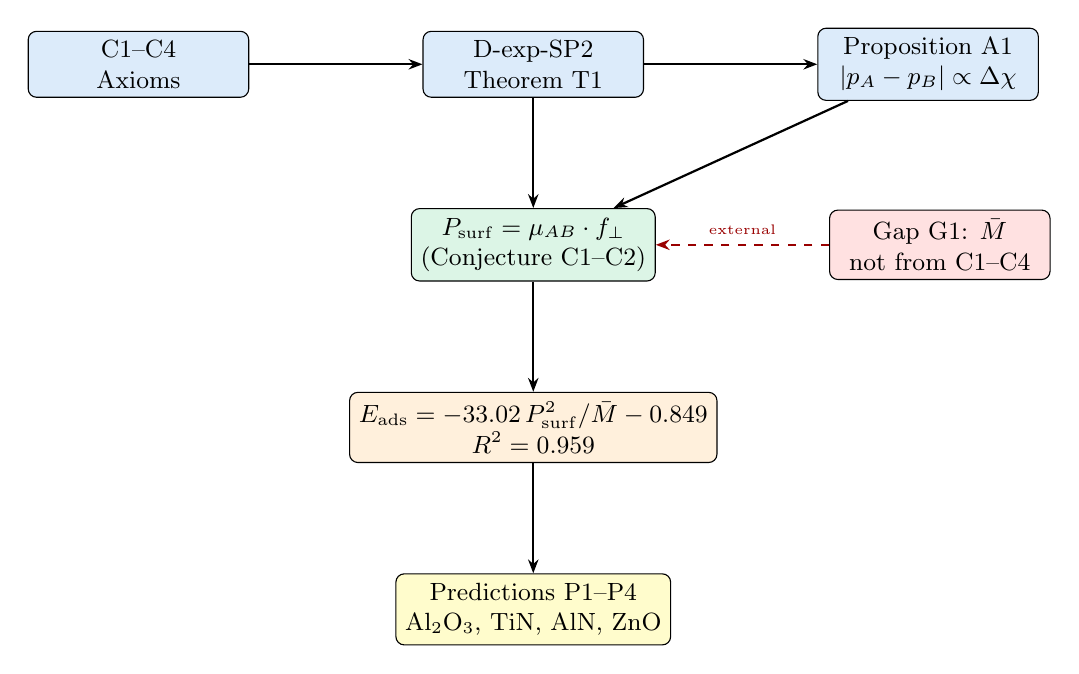
\begin{tikzpicture}[
  node distance=1.4cm and 2.2cm,
  box/.style={draw, rounded corners=3pt, minimum width=2.8cm,
              minimum height=0.8cm, align=center, font=\small},
  arr/.style={-{Stealth[length=5pt]}, thick}]

\node[box, fill=pdllightblue]  (C14)  {C1--C4\\Axioms};
\node[box, fill=pdllightblue,  right=of C14] (SP2) {D-exp-SP2\\Theorem T1};
\node[box, fill=pdllightblue,  right=of SP2] (A1)  {Proposition A1\\$|p_A-p_B|\propto\DeltaEN$};
\node[box, fill=pdllightgreen, below=of SP2] (Psurf) {$\Psurf = \muAB\cdot\fracZ$\\(Conjecture C1--C2)};
\node[box, fill=pdllightorange, below=of Psurf] (Reg) {$\Eads=-33.02\,\Psurf^2/\Mmoy-0.849$\\$R^2=0.959$};
\node[box, fill=yellow!20,     below=of Reg] (Pred) {Predictions P1--P4\\Al$_2$O$_3$, TiN, AlN, ZnO};
\node[box, fill=pdllightred,   right=of Psurf] (G1)  {Gap G1: $\Mmoy$\\not from C1--C4};

\draw[arr] (C14) -- (SP2);
\draw[arr] (SP2) -- (A1);
\draw[arr] (SP2) -- (Psurf);
\draw[arr] (A1)  -- (Psurf);
\draw[arr] (Psurf) -- (Reg);
\draw[arr] (Reg) -- (Pred);
\draw[arr, dashed, red!60!black] (G1) -- (Psurf) node[midway, above, font=\tiny]{external};
\end{tikzpicture}
\end{center}

%% ════════════════════════════════════════════════════════════════════════════
\section{Discussion and Outlook}

\subsection{Scope and Limitations}

The selection principle Eq.~\eqref{eq:model} is validated on 9 materials across three crystal families. Its domain of validity is physisorption on polar semiconductor and ionic surfaces in the wurtzite, zinc-blende, and rocksalt families. It does not apply to layered hexagonal structures (BN, graphite: $\fracZ = 0$) without modification, nor to systems where chemisorption dominates (MgO at the MACE level of theory).

The \MACE\ simulation uses neutral atoms. The true $\Eads$ of Zn$^{2+}$ in aqueous solution involves a desolvation penalty of $+2$ to $+4$\,eV per ion, largely cancelling the negative adsorption energy. The experimental $\Csp$ depends on the balance between adsorption energy and desolvation energy — a quantity not computed here. The predictions P1--P4 are therefore conditional on the desolvation penalty being approximately constant across candidates, which is reasonable for aqueous ZnSO$_4$ at equal ionic strength.

\subsection{Next Steps}

Three directions are open. First, experimental validation of P1--P4 by any group with access to nanoparticulate Al$_2$O$_3$ or AlN and a standard three-electrode \EIS\ setup in ZnSO$_4$. Second, formal derivation of the Mulliken correspondence (Gap~G2) within the PDL spectral framework — extending Proposition~A1 from the 2-node graph to the full supercell. Third, DFT-level NEB calculations for Zn$^{2+}$ diffusion on Al$_2$O$_3$ and TiN surfaces, to confirm the physisorption mechanism and rule out lattice intercalation.

\subsection{Relation to the Corpus}

This document is classified exploratory (D-exp). Its theorems are inherited from D-exp-SP2 and D49. Its conjectures do not invalidate any established corpus result. The negative result on bulk diffusion (Section~\ref{sec:bulk}) is consistent with the PDL bipartite criterion, which governs electronic coherence, not ionic mobility.

%% ════════════════════════════════════════════════════════════════════════════
\section{Conclusion}

We have derived a materials selection principle for zinc-ion aqueous supercapacitor electrodes from the PDL bipartite bond graph criterion. The descriptor $\Psurf^2/\Mmoy$, where $\Psurf = d_{AB}\sqrt{\DeltaEN}\cdot\fracZ$ is the surface dipole moment, predicts the Zn adsorption energy with $R^2 = 0.959$ across nine materials of three crystal families. The quantity $\DeltaEN$ is partially derivable from the bond graph spectral structure (Proposition~A1, $r = 0.988$). The mass parameter $\Mmoy$ plays the structural role of $\Delta m_{\mathrm{iso}}$ in the PDL nuclear programme — forced by the heteratomic bipartite structure, irreducible from combinatorial axioms alone (Gap~G1).

Priority experimental candidates are Al$_2$O$_3$, TiN, AlN, and ZnO nanoparticles in ZnSO$_4$ aqueous electrolyte, with falsifiable specific capacitance predictions. The exchangeable cartridge architecture leverages the sub-minute recharge time of supercapacitors and the chemical stability of all active materials.

%% ── Remerciements ─────────────────────────────────────────────────────────
\section*{Acknowledgements}

The author thanks the open-access communities of Materials Project, MACE-MP, and pymatgen for the computational infrastructure on which this work relies. All numerical results are fully reproducible from the Python scripts deposited alongside this document on Zenodo.

\clearpage

%% ── Références ────────────────────────────────────────────────────────────
\bibliographystyle{unsrt}
\bibliography{D-exp-ZIB}

\end{document}
